Wir haben uns bei der Entwicklung im Vorhinein Gedanken über die Aufteilung im Design gemacht. Dies ist sehr wichtig, um schlussendlich eine übersichtliche Anwendung zu haben. Des weiteren war diese Entscheidung in unserem Fall sehr wichtig, da das Kundenmanagement Tool übersichtlich sein muss, um die Schnelligkeit in der Benutzung zu maximieren.
Aus diesem Grund haben wir uns für folgende Aufteilung entschieden:

\begin{figure}[h!]
    \centering
    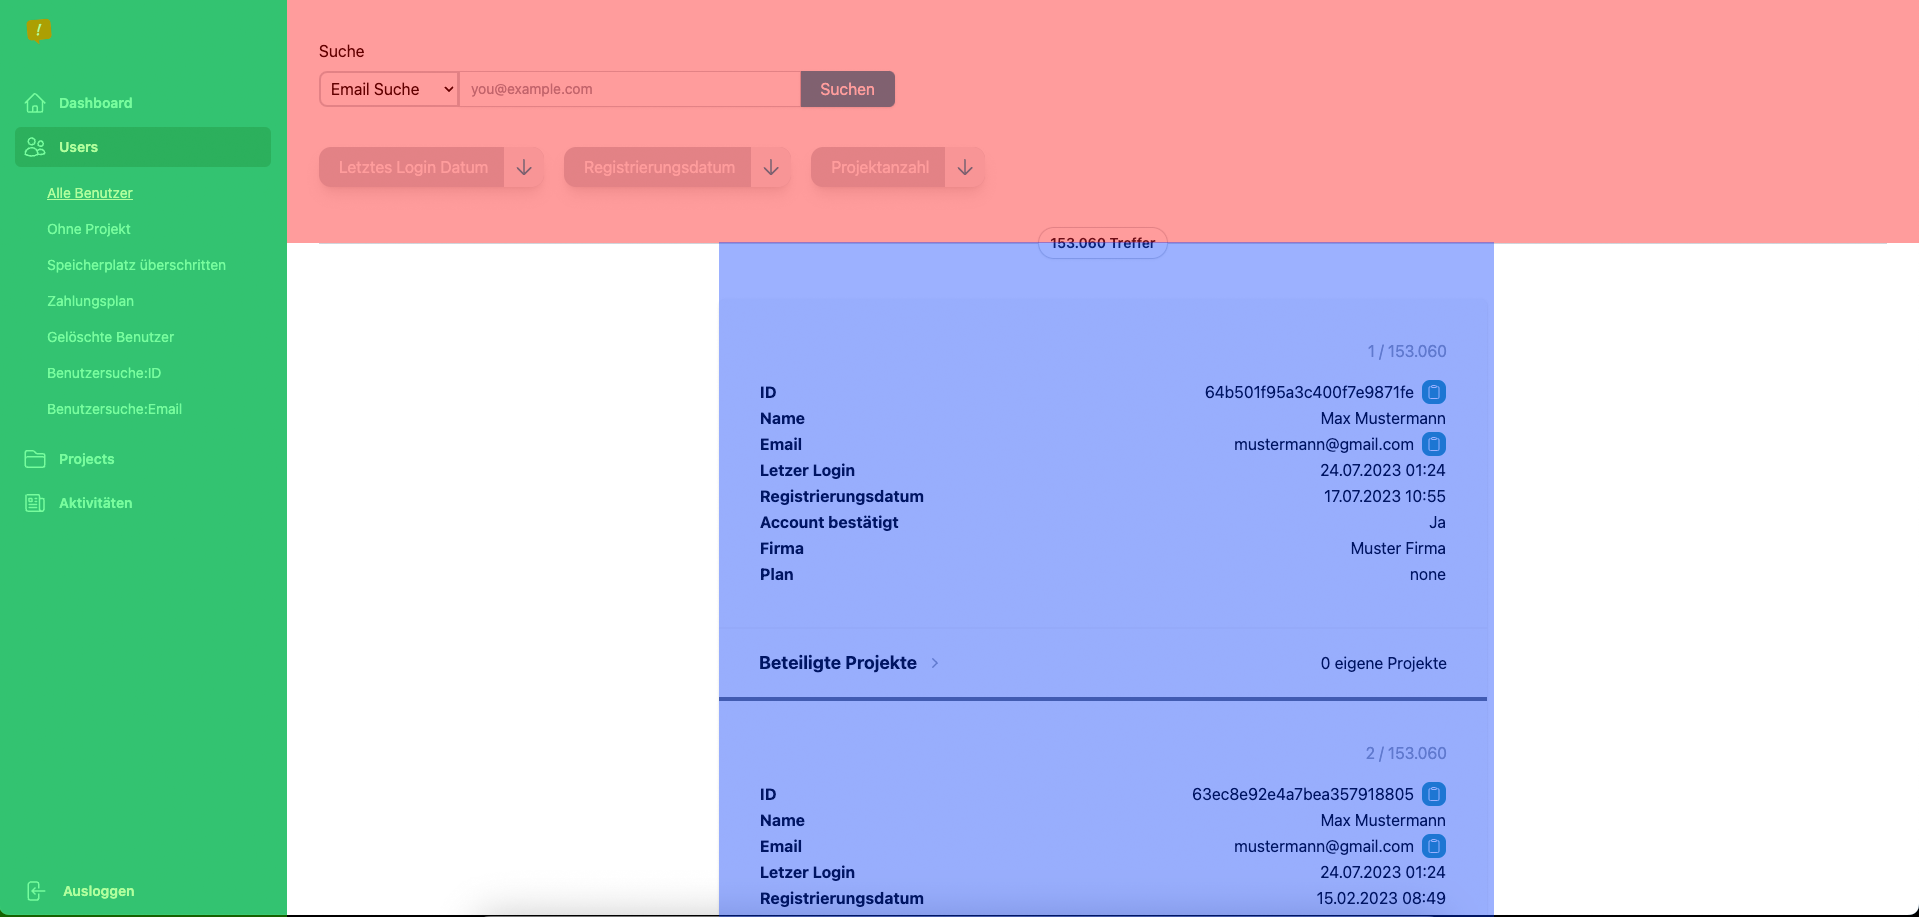
\includegraphics[width=1\textwidth]{pics/planfred-grids.png}
    \caption{Kundenmanagement Tool Layout}
    \label{fig:mesh1}
\end{figure}

Wie an der Grafik zu sehen ist, ist das Layout grundsätzlich in 3 Bereiche aufgeteilt. Der grüne Bereiche symbolisiert den Bereich in dem sich die Navigation befindet. Der rote Bereiche stellt die Breite da, die dann noch zur Verfügung steht.

Diesen ganzen Bereich haben wir bewusst verwendet um Elemente zu positionieren, wie Suchleiste oder Buttons zum sortieren der Ergebnisse. Diese haben somit einen eigenen Bereich, sind klar erkenntlich und leicht zu verwenden. Ebenfalls ist diese Section immer oben auf einer Seite platziert.

Die letzte Section ist hierbei der blaue Bereich. Dieser ist dazu da, um die Ergebnisse beziehungsweise den tatsächlichen Content darzustellen. Dieser verwendet nicht die ganze zur Verfügung stehende Breite, sondern ist beschränkt. Die Breite war dabei eine bewusste Entscheidung, damit die Benutzer:innen die Ergebnisse auf einen Blick sehen können und nicht die ganze Breite abscannen müssen. Das sorgt für eine bessere Übersicht und beschleunigt den Prozess den richtigen User oder Projekt zu finden.

